

The hardware consists of network cameras connected directly by Ethernet to a processing unit. The system should be able to handle cameras with a resolution of at least 2M pixel. The cameras are connected to the processing unit a network or USB. 
The processing unit is a computer connected to one or more cameras that displays the calculated results. 

\begin{figure}[htb]
	\centering
	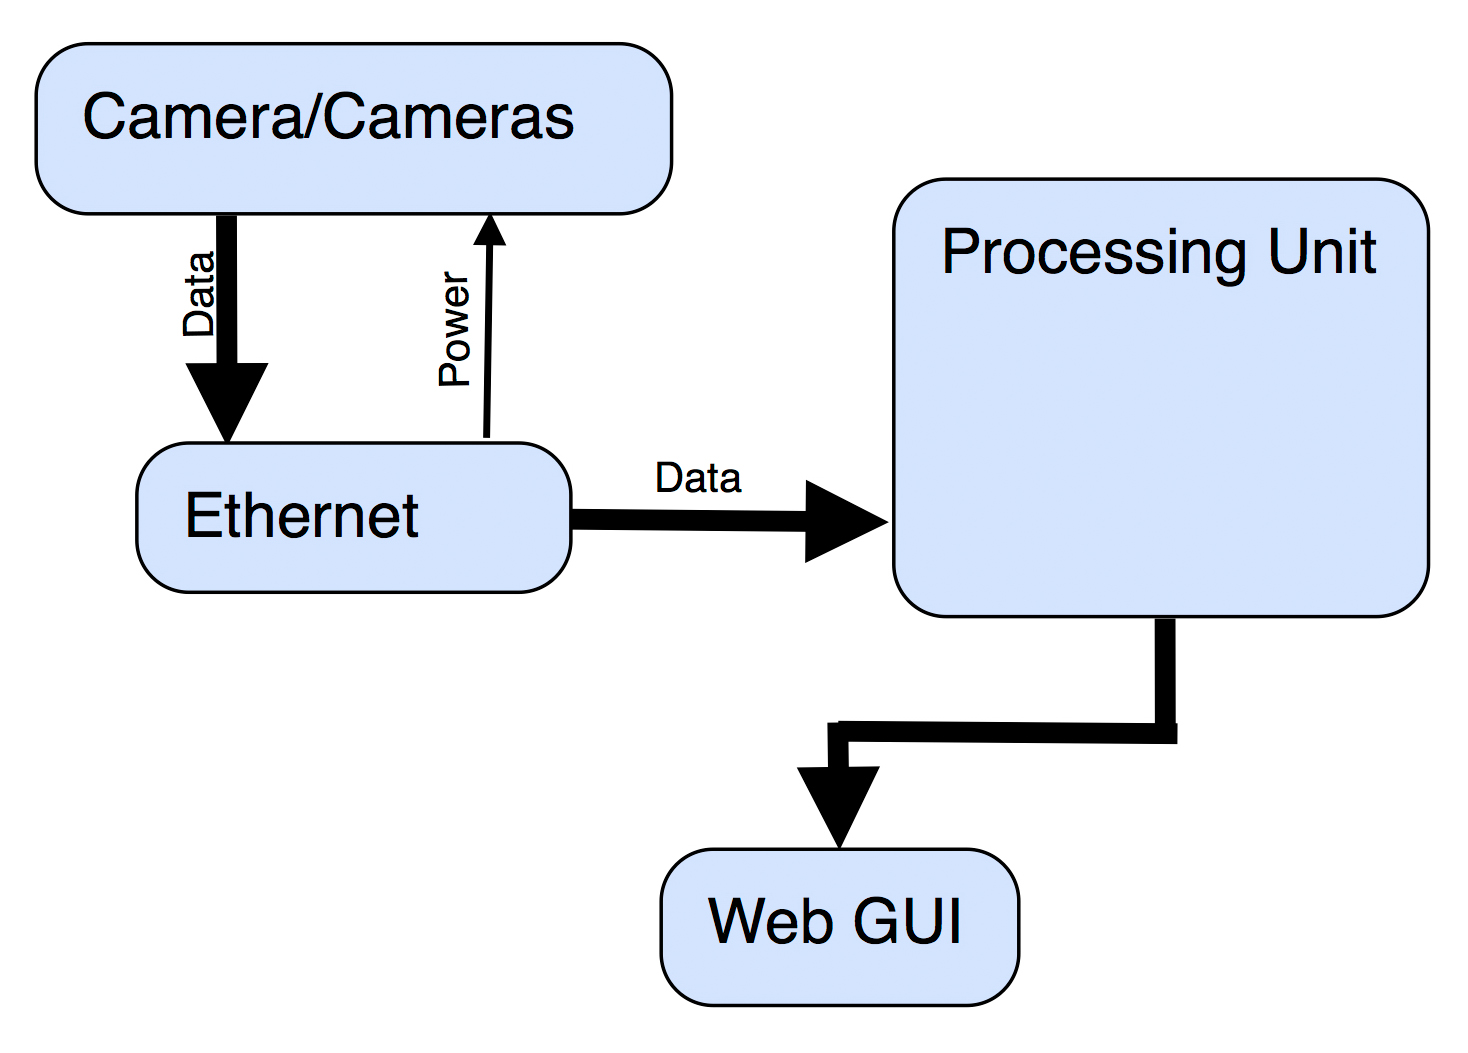
\includegraphics[width=160mm]{images/Hardware-flowchart.jpg}
	\caption[This text ends up at the list of figures]{\textit{Flowchart hardware modules}}
	\label{fig:block_overview_fig}  %Skapar referens till figuren
\end{figure}


\subsection{Limitations}
The hardware is limited by budget, Internet connection and the source of power. The cost is limited to approximately 15.000 SEK per room, including installation costs. The budget limits performance of the cameras e.g. resolution and number of cameras. The connection to the cameras need to be stable and have a bandwidth good enough for sending live video from the cameras.   
\newpage
\subsection{Hardware Requirements}
\label{sec:hardware_req}
\reqtable
{
	\addreq{The system uses network cameras powered via Ethernet.\newline \textbf{Revised 2013-11-13:} The system uses cameras connected to a laptop (mid-end processing device) via network or USB.}{1}	
	\addreq{The system can operate using high resolution ($>$2 Mpixel) cameras}{1}
	\addreq{Lower resolution cameras can be used}{2}
	\addreq{The application can run using the processing power provided by the costumer.\newline \textbf{Canceled 2013-11-13: }No processing power is provided by the customer.}{--}
	\addreq{The application can run using a mid-end processing device.\newline \textbf{Revised priority 2013-11-13:} The cancellation of previous req.(\textbf{3.4}) causes priority to change \textbf{from 2 to 1.}}{1}
	\addreq{The application can run using a low-end processing device.}{3}
}